\chapter{Démarche utilisée}

Ce chapitre présente la démarche utilisée aussi bien pour la gestion de notre projet que notre façon d'aborder le développement technique de la solution réalisée.

\section{Gestion de projet}

Au cours de ces trois semaines, afin d'atteindre l'objectif fixé, il était essentiel d'avoir des bonnes méthodes de gestion de projet. Dans cette partie, nous expliquons les méthodes mises en oeuvre pour dans le cadre de cette gestion de projet.

\subsection{Planification}

Une des premières étape de la gestion de projet a été de planifier ces trois semaines. Cette étape permet de déterminer et surtout d'ordonnancer les tâches à réaliser pendant le projet. Elle permet également d'estimer leurs charges.\\

Pour mener à bien cette étape de réalisation, nous avons choisi de mettre en oeuvre un Gantt. Ce Gantt permet :

\begin{itemize}
    \item Déterminer si les objectifs sont réalisés ou dépassés
    \item Suivre et communiquer l’avancement du projet
    \item Affecter les ressources aux tâches

\end{itemize}

Le Gantt prévisionnel est disponible sur la figure~\ref{fig:gantt_prev}

\begin{figure}[!ht]
\begin{center}
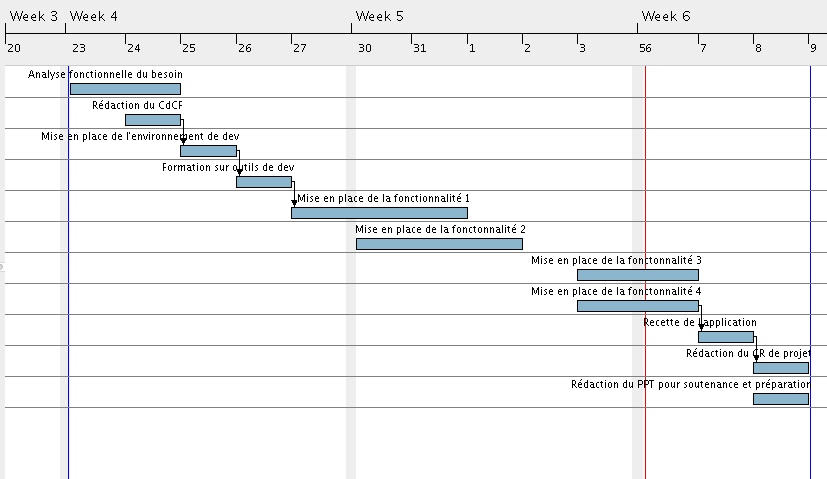
\includegraphics[scale = 0.3]{img/gantt-prev.png}
\end{center}
\caption{Gantt Prévisionnel}
\label{fig:gantt_prev} 
\end{figure}

Le Gantt réel est disponible sur la figure ..

\section{Gestion du développement technique}

Dans cette partie, nous expliquons la façon dont nous avons procédé pour gérer le développement technique de l'application.

\subsection{Installation des outils de développement}

La première partie a été l'installation des nouveaux composants nécessaires aux développement d'une application sur l'environnement de CozyCloud. Ces éléments sont ceux cités dans la partie 3.1.2.1.


\subsection{Formation sur l'outil CozyCloud}

C'est une des parties qui nous a pris le plus de temps. En effet, nous ne connaissions par du tout l'environnement de développement, et nous avons fait face à un manque accru de documentation.

Nous avons donc sollicité les développeurs de chez Cozy, directement sur un tchat mis à disposition (IRC channel #cozycloud). Cela nous a permis d'en apprendre davantage sur la plateforme, mais cela nous a également permis, une fois le développement commencé, d'aider à la résolution de nos divers problèmes.

\subsection{Développement des fonctionnalités}

Pour le développement des fonctionnalités, nous nous sommes appuyés sur plusieurs API disponibles. Ainsi, nous avons pu utiliser l'API cozybrowser-sdk. Il a donc fallu par commencer par lire les documentations. \\

Aussi, nous nous sommes aidés d'un tuto "Make a client side-app..." disponible sur le site de cozy-cloud. Il nous a permis de prendre nos repères sur le développement d'application client-side et de débuter la programmation de notre application My Portfolio.